\documentclass[10pt,a4paper]{article}
\usepackage[utf8]{inputenc}
\usepackage[T1]{fontenc}
\usepackage[polish]{babel}
\usepackage{graphicx}
\usepackage{polski}
\usepackage{listings}

\title{Kolokwium z Technologi Informacyjnych 2019}
\author{Imię i Nazwisko, grupa XX}

\begin{document}
	
	\maketitle
	
	\tableofcontents
	
	\section{Zdjęcia piesków w \LaTeX}
	
	Rysunek \ref{dog} przedstawia zdjęcie bardzo uśmiechniętego pieska.
	
	\begin{figure}[h]
		\centering
		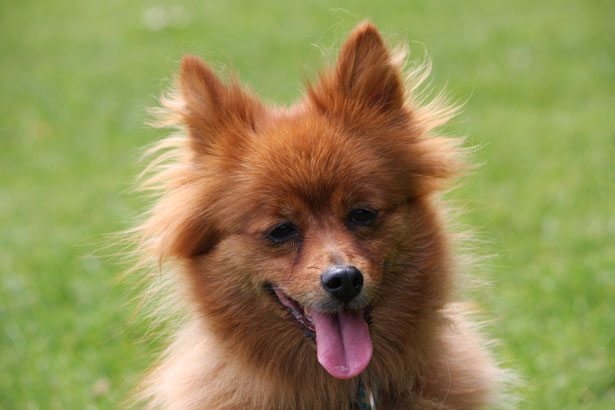
\includegraphics[width=0.5\textwidth]{pies.png}
		\caption{Zdjęcie wesołego pieska, wyśrodkowane i zajmujące połowę szerokości tekstu}
		\label{dog}
	\end{figure}

	\section{Tabelaryczna lista uczniów}
	
	Tabela \ref{uczniowie} umieszczona jest w otoczeniu pływającym i jest wycentrowana.
	
	\begin{table}[h!]
		\centering
		\begin{tabular}{c | c || c}
			\hline
			\multicolumn{3}{c}{Uczniowie} \\ \hline \hline
			Imię & Nazwisko & Nr. w dzienniku \\ \hline
			Jan & Kowalski & 1 \\
			Krystian & Pierwszaławka & 6 \\
			Olek & Nadosiadkę & 7 \\
			Maria & Znana & 2 \\
		\end{tabular}
		\caption{Lista uczniów, wraz z numerami w dzienniku}
		\label{uczniowie}
	\end{table}

	\section{Prezentacja wyników matematycznych}
	
	\subsection{Wzór na krzywą Gaussa}
	
	Poniżej przedstawiono wzór opisujący krzywą Gaussa w zależności od dwóch parametrów, $\mu$ - średniej i $\sigma$ - odchylenia:
	
	\begin{equation}
		g(x) = \frac{1}{\sigma \sqrt{2 \pi}}e^{-\frac{1}{2}\left(\frac{x-\mu}{\sigma}\right)^2}
	\end{equation}
	
	\subsection{Wykres trzech krzywych Gaussa}
	
	Na Rysunku \ref{wykres} widzimy wykres będący sumą trzech krzywych Gaussa o następujących parametrach:
	\begin{enumerate}
		\item $\mu = -1$, $\sigma = 0,5$
		\item $\mu = 0$, $\sigma = 1$
		\item $\mu = 2$, $\sigma = 3$
	\end{enumerate}

	\begin{figure}[h]
		\centering
		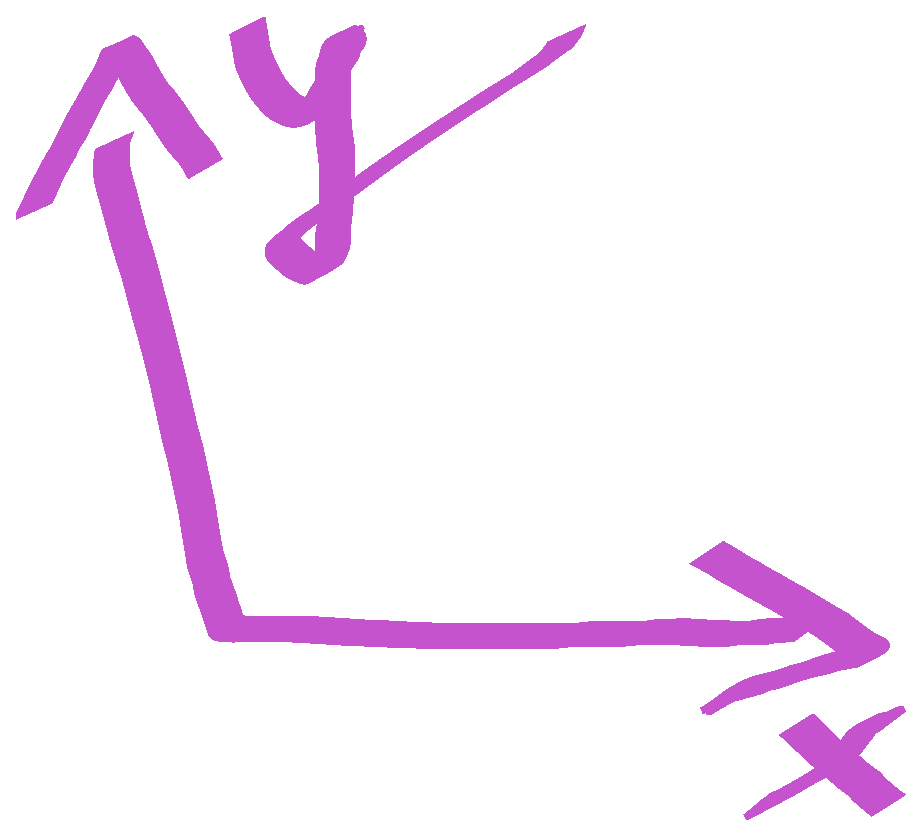
\includegraphics[width=0.5\textwidth]{wykres.eps}
		\caption{Wykres sumy trzech krzywych Gaussa, zajmuje połowę szerokości tekstu}
		\label{wykres}
	\end{figure}

	\subsection{Kod źródłowy}
	
	Poniżej znajduje się kod źródłowy, który pozwala wygenerować wykres z Rysunku \ref{wykres}:
	
	\begin{lstlisting}[language=matlab]
%TUTAJ WSTAW KOD ZRODLOWY, KTORY NAPISZESZ REALIZAUJAC ZADANIE 1

plot(x, y);

disp('Bardzo wazna wiadomosc')
	\end{lstlisting}
	
\end{document}